\documentclass[letterpaper]{article}
\usepackage{graphicx}                    % PNG images
\usepackage{wrapfig}                     % Wrap text around images
\usepackage[usenames,dvipsnames,table]{xcolor} % Colors
% [Basic names, postscript predefined names, allow colored table backgrounds]
\usepackage[margin=0.5in]{geometry}      % Easy way to set margins
\usepackage{multirow}                    % Allow "merged cells" in tables
\usepackage{wasysym}                     % Male and Female symbols
\usepackage{etoolbox}                    % Conditionals like \ifstrequal
\usepackage{rotating}                    % Allow sideways text
\usepackage[absolute]{textpos}           % Allows arbitrarily-positioned text
\setlength{\TPHorizModule}{1em}          % X grid unit for textpos
\setlength{\TPVertModule}{\TPHorizModule}% Y grid unit for textpos
\usepackage{changepage}                  % Adjustwidth environment
\usepackage{xparse}                      % Multi-default argument commands, etc
\usepackage{tabu}                        % Ultra-flexible tabular replacement

% Default to not indenting any paragraphs, but allow \indent to still work
\newlength\tindent
\setlength{\tindent}{\parindent}
\setlength{\parindent}{0pt}
\renewcommand{\indent}{\hspace*{\tindent}}

% Styles
\newcommand{\colhead}[0]{\footnotesize\itshape}
\newcommand{\e}[1]{\emph{#1}}
\newcommand{\B}[1]{\textbf{#1}}

% Shorthand for math mode commands
\newcommand{\s}[0]{$^S$}
\newcommand{\N}[0]{$^N$}
\newcommand{\D}[0]{$^\dag$}

% Color for rotated text in spellbook
\definecolor{light-gray}{RGB}{179,179,179}
% Background color for table rows, equal to pathfinder logo
\definecolor{tan}{RGB}{228, 220, 147}

% Command to print a skill row
\newcommand{\skill}[4]{\B{#1} & #2 & {\footnotesize{#3}} & #4 \\}

% Command to clean up rows in inventory
\NewDocumentCommand{\thing}{ s m O{} }{
    \IfBooleanTF{#1}{\hspace{1em} #2 & #3\\}{#2 & #3\\}}

% Command to print sideways text in spellbook left margin
\newcommand{\spelllevel}[2]{
\begin{textblock}{1}(0.5,#1)
\begin{sideways}
     {\color{light-gray}{\LARGE \e{#2}}}
\end{sideways}
\end{textblock}}

% Command to print a spell with all sorts of pretty formatting and a
% checkbox to the left
\newcommand{\spell}[7]{
\begin{wrapfigure}{l}{2em}
\vspace{-13pt}
\ifstrequal{#2}{Full}{  
\includegraphics[width=2em]{Checkbox-Full}}{
\ifstrequal{#2}{Scroll}{
\includegraphics[width=2em]{Checkbox-S}}{
                        
\includegraphics[width=2em]{Checkbox}}}
\ifstrequal{#7}{}{\vspace{-1em}}{\vspace{#7}}
\end{wrapfigure}
 \B{#1} #3 {
    \ifstrequal{#4}{Conj}{\color{Plum}Conj}{%
    \ifstrequal{#4}{Divin}{\color{YellowOrange}Divin}{%
    \ifstrequal{#4}{Ench}{\color{VioletRed}Ench}{%
    \ifstrequal{#4}{Trans}{\color{LimeGreen}Trans}{%
    \ifstrequal{#4}{Evoc}{\color{RedOrange}Evoc}{%
    \ifstrequal{#4}{Illu}{\color{ProcessBlue}Illu}{%
    \ifstrequal{#4}{Abjur}{\color{CadetBlue}Abjur}{%
    \ifstrequal{#4}{Necro}{\color{Red}Necro}{%
}}}}}}}}}
{\footnotesize \e{#5}} \\
#6
}

% Environment with smaller font started with huge title and line
\newenvironment{notesection}[1]
{ {\huge \B{#1}}\hrule\vspace{0.5em}\begingroup\fontsize{9pt}{12pt}\selectfont}
{\endgroup}

% Command to print a person with a colored M/F symbol
\newcommand{\person}[3]{\B{#1
    \ifstrequal{#2}{M}{{\color{ProcessBlue}\male}}{%
    \ifstrequal{#2}{F}{\color{VioletRed}\female}{}}}{\scriptsize #3}}


\begin{document}
\sffamily
\begin{wrapfigure}{r}{13em}
\vspace{-1.5em}
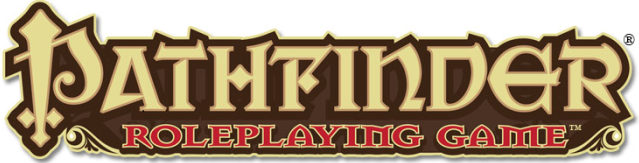
\includegraphics[width=13em]{Pathfinder}
\end{wrapfigure}
 \B{\huge{Trostram }\Large{Human Magus 2}} \\
\e{Chaotic Good} \hspace{2em} \e{Age 24y} \hspace{2em} \e{Height 5ft 3in} \hspace{2em} \e{Weight 135lb} \par
% Hair Red-Brown, Eyes Green
\hrule

\begin{tabu} to 0.333\textwidth{X[4] X[1c] X[1c]}
\multicolumn{3}{c}{\e{Ability Scores}} \\
\B{Strength} & 19  & +4 \\
\B{Dexterity} & 12 & +1 \\
\B{Constitution} & 13 & +1 \\
\B{Intelligence} & 18 & +4 \\
\B{Wisdom} & 9 & -1 \\
\B{Charisma} & 10 & +0 \\
\end{tabu}
%
\begin{tabu} to 0.333\textwidth{X[5] X[1c]}
\multicolumn{2}{c}{\e{Defenses}} \\
\B{Armor Class} & 14 \\
Touch & 11 \\
Flat Footed & 13 \\
\B{Fortitude} & 4 \\
\B{Reflex} & 1 \\
\B{Will} & 2 \\
\end{tabu}
%
\begin{tabu} to 0.333\textwidth{X[5] X[1c]}
\multicolumn{2}{c}{\e{Movement}} \\
\B{Speed} & 30 ft \\
\B{Initiative} & +1 \\ 
\multicolumn{2}{c}{~} \\
\multicolumn{2}{c}{\e{Health}} \\
\B{Hit Points} & 12 \\ % Max at lvl 1, 2 at level 2, +1xlvl CON, +2 favored class
Current HP & 2 \\
\end{tabu}
%
\begin{tabu} to 0.5\textwidth{X[7] X[1c] X[2c] X[2c]}
\multicolumn{4}{c}{\e{Attacks and Damage}} \\
\rowfont{\colhead}Name & Bonus &&\\
\taburowcolors 2{tan..white}
\B{Base Attack Bonus} & +1 && \\
\B{Combat Maneuver} & +5 && \\ % BAB + STR + 1 if small
\B{Combat Defense} & 16 && \\ % BAB + STR + DEX + 1 if small + 10
\B{M\^{e}l\'{e}e Touch Attack} & +5 && \\
\B{Ranged Touch Attack} & +2 && \\ 
\taburowcolors 2{white..white}
\\
\rowfont{\colhead}Name & Bonus & Damage & Critical \\
\taburowcolors 2{tan..white}
\B{Longsword} & +6 & 1d8+4 & 19-20x2 \\
\multicolumn{4}{l}{\e{Slashing}} \\
\taburowcolors 2{white..white}
\\\\\\\\\\\\\\\\\\\\\\
\end{tabu}
%
\begin{tabu} to 0.5\textwidth{X[9] X[2c] X[2c] X[2c]}
% 2+INT mod/level +0 for favored class 0 times +2 for skilled racial trait = 14 ranks
\\
\multicolumn{4}{c}{\e{Skills}} \\
\rowfont{\colhead}Name & Bonus & Ability & Ranks \\
\taburowcolors 2{tan..white}
\skill{Acrobatics}{1}{DEX}{-}
\skill{Appraise}{4}{INT}{-}
\skill{Bluff}{0}{CHA}{-}
\skill{Climb}{8}{STR}{1}
% Not a skill, but a CL + INT check; "ranks" actually CL here
\skill{Concentration}{6}{INT}{2}
%\skill{Craft {\scriptsize CLOTH}}{9}{INT}{1}
\skill{Diplomacy}{1}{CHA}{1}
%\skill{Disable Device*}{-}{DEX}{-}
\skill{Disguise}{0}{CHA}{-}
\skill{Escape Artist}{1}{DEX}{-}
\skill{Fly}{1}{DEX}{-}
%\skill{Handle Animal*}{-}{CHA}{-}
\skill{Heal}{2}{WIS}{1}
\skill{Intimidate}{0}{CHA}{-}
\skill{Knowledge {\scriptsize ARCANA}*}{8}{INT}{1}
\skill{Knowledge {\mbox {\scriptsize DUNGEONEERING}*}}{8}{INT}{1}
%\skill{Knowledge {\scriptsize ENGINEERING}*}{-}{INT}{-}
%\skill{Knowledge {\scriptsize GEOGRAPHY}*}{-}{INT}{-}
%\skill{Knowledge {\scriptsize HISTORY}*}{15}{INT}{7}
%\skill{Knowledge {\scriptsize LOCAL}*}{-}{INT}{-}
%\skill{Knowledge {\scriptsize NATURE}*}{-}{INT}{-}
%\skill{Knowledge {\scriptsize NOBILITY}*}{9}{INT}{1}
\skill{Knowledge {\scriptsize PLANES}*}{8}{INT}{1}
%\skill{Knowledge {\scriptsize RELIGION}*}{-}{INT}{-}
%\skill{Linguistics*}{-}{INT}{-}
\skill{Perception}{1}{WIS}{2}
\skill{Perform}{0}{CHA}{-}
%\skill{Profession*}{-}{WIS}{-}
\skill{Ride}{1}{DEX}{-}
\skill{Sense Motive}{1}{WIS}{2}
\skill{Spellcraft*}{9}{INT}{2}
\skill{Stealth}{2}{DEX}{1}
\skill{Survival}{-1}{WIS}{-}
\skill{Swim}{8}{STR}{1}
%\skill{Use Magic Device*}{-}{CHA}{-}
\multicolumn{4}{l}{\footnotesize * Trained Only} \\
\end{tabu}
\tabureset
%
\e{Feats}\\
\B{Arcane Strike} Swift action: grant your weapon a +1 to damage (affected weapon treated as magic in terms of damage reduction). \\ %+2/+3/+4/+5 at level 5/10/15/20
\B{Combat Casting} +4 on concentration checks to cast defensively. \\
\\
\e{Traits and Special Abilities (Source)} \\
\B{Skilled} +1 skill rank per level (Race) \\
\B{Bonus Feat} One extra feat at first level (Race) \\
\B{Inspired} Once per day, take the higher of two rolls on a skill check (Trait) \\
\B{Swordsman's Page} +1 on critical confirmation rolls with a longsword (Trait) \\
\B{Arcane Pool} 5 points available. For 1 point, as a swift action, held weapon gains a +1 enhancement bonus for 1 minute. (Class) \\%1/2 level+INT points in pool. +1/+2/+3/+4/+5 bonus at level 1/5/9/13/17, not to exceed +5 when added to existing enchantment, Other options at 5th level
\B{Spell Combat} When wielding a light or one-handed m\^{e}l\'{e}e weapon, as a full-round action, make all attacks with the weapon at a -2 penalty and simultaneously cast any standard action spell (if it requires an attack, it also takes the -2). If casting defensively, may opt to take up to an additional -4 on the attack and add that amount to the concentration check. (Class)\\ %Up to INT modifier additional penalty/bonus
\B{Spellstrike} When casting a touch spell, instead of receiving a free touch attack as part of casting, you may opt to deliver it as part of a free m\^{e}l\'{e}e attack (not a touch attack). 
\\
\e{Languages} \\
\B{Common, Draconic, Dwarven, Elvish, Goblin} \\
\\
{\e{Experience}} \\
\B{2,400 / 5,000} \\
\\
{\e{Wealth}} \\
\B{53g 7s 9c}

\pagebreak
\B{\huge{Inventory}}
\hrule
\begin{tabu} to 0.5\textwidth[h]{X[3] X[1c]}
    \multicolumn{2}{c}{\e{Personal Gear}}\\
    \taburowcolors 2{tan..white}
    \thing{Explorer's Outfit}[8]
    \thing{Studded Leather}[20]
    \thing{Longsword}[4]
    \thing{Spell Component Pouch}[2]
    \thing{Masterwork Backpack}[4]
    \thing*{Spellbook}[3]
    \thing*{Journal}[1]
    \thing*{Ink, Inkpen}
    \thing*{Soap}[1]
    \thing*{5 Days' Trail Rations}[5]
    \thing*{5 pt Lamp Oil}[5]
    \thing*{}[]
    \thing{Waterskin}[4]
    \thing{Small Tent}[20]
    \thing{Bedroll}[5]
    \thing{Hooded Lantern}[2]
    \taburowcolors 2{white..white}
    \thing{}[\B{84/133}]
    \multicolumn{2}{r}{Med 266, Heavy 400, Lift 800, Push/Drag 2000}
\end{tabu}
\begin{tabu} to 0.5\textwidth[h]{X[3] X[1c]}
    \multicolumn{2}{c}{\e{Party Loot and Supplies}}\\
    \taburowcolors 2{tan..white}
    &\\&\\&\\&\\&\\&\\
    &\\&\\&\\&\\&\\&\\
    &\\&\\&\\&\\&\\&\\
    \taburowcolors 2{white..white}
\end{tabu}
%
\begin{tabu} to 0.5\textwidth[h]{X}
    \e{Party Members} \\
    \B{Trostram} Human Magus 1 (Ryan) \\
    \B{Geoffrey} Human Summoner 1 (Jeremy) \\
    \B{Tom} Human Monk 1 (Mikey) \\
    \B{Khrili} Half-Elf Witch 1 (JT) \\
\end{tabu}

\pagebreak

\spelllevel{14}{Cantrips}
\spelllevel{35}{First: 2/day}

{\huge \B{Spellbook}} \hspace{2em}4/3 per day\par
\hrule\vspace{0.5em}

\spell{Detect Magic}{Full}{V S}{Divin}{Standard Action / 60ft range / 7 minute duration (D)}{
Detect magic auras in a cone-shaped emanation.  Concentrate longer to reveal more detailed information:\\
\e{1st Round}: Presence or absence of auras.\\
\e{2nd Round}: Number of auras, strength of most potent aura.\\
\e{3rd Round}: Strength and location of each aura.  For each aura, a successful Knowledge (arcana) check determines the school of the aura (DC 15 + spell level or +1/2 caster level on non-spells); a successful Spellcraft determines the properties of magic items (DC 15 + caster level).}{3em} %1min/lvl

\spell{Mage Hand}{Full}{V S}{Trans}{Standard Action / 40ft Range / concentration duration}{%
Manipulate an object at a distance. As a move action, move the object up to 15 feet in any direction.\\}{}\\[-2em] % Close (25ft+5ft/2lvl)

\spell{Ray of Frost\D}{Full}{V S}{Evoc}{Standard Action / 40ft Range / Instant}{
With a successful ranged touch attack, a ray of ice strikes the target for 1d3 cold damage.\\}{}\\[-2em] % Close (25ft+5ft/2lvl)

\spell{Read Magic}{Full}{V S F (a clear crystal prism)}{Divin}{Standard Action / Personal / 70 minutes*}{
You can decipher magical inscriptions; doing so does not invoke the magic contained in the writing.  After reading a particular inscription, you are thereafter able to read it again without this spell.  You can read about one page per minute. Allows identification of a \e{glyph of [greater] warding} with DC 13[16] Spellcraft check, or any \e{symbol} spell with a Spellcraft of DC 10 + the spell level.}{1em}\\[-1em] %10min/lvl
\begin{adjustwidth}{3em}{0em}
Others: \B{Acid Splash, Arcane Mark, Dancing Lights, Daze, Disrupt Undead, Flare, Ghost Sound, Light, Open/Close, Prestidigitation, Spark}\\
\end{adjustwidth}

%LVL2: Add 2 more level 1 spells known

\spell{Expeditious Retreat}{}{V S}{Trans}{Standard Action / Personal / 1 minutes (D)}{%
Increases your base land speed by 30ft.}{}\\[-1em] %1min/lvl

\spell{Mirror Strike}{}{V S M (shard of a mirror)}{Trans}{Standard Action / Personal}{%
Next attack roll may hit two targets in reach; +2 attack if targets have flanking on you. If the attack hits both, each takes half damage; if it hits one, deal damage to it as normal. A critical threat is only confirmed if the confirmation roll hits both.}{}\\[-1em]

\spell{Shock Shield}{}{V S}{Abjur}{Standard Action / Self / 1 minute duration (D)}{%
Negates \emph{magic missiles} targeted at you; +2 shield bonus to AC. Dismissing deals 1d6 electrical damage to creatures in a 5 foot burst (Ref DC 15 half).}{}\\[-1em] %1min/lvl

\spell{Shocking Grasp}{}{V S}{Evoc}{Standard Action / Touch / Instant}{%
Touch delivers 1d6 electricity damage; +3 on the attack if target is wearing metal armor.}{}\\[-1em] %1d6/level, max 5d6

\spell{True Strike}{}{V F (small wooden replica of an archery target)}{Divin}{\mbox{Standard Action / Personal / See Text}}{%
\mbox{Your next single attack gains a +20 insight bonus, and is not affected by miss change from striking a concealed target.}}{}\\[-1em]

\spell{Unerring Weapon}{}{V S}{Trans}{Standard Action / 25ft Range / 1 Round}{%
Target weapon (or 20 projectiles) gain +2 on critical confirmation rolls.}{}\\[-1em] %Close (25ft+5ft/2lvl), 1 Round/level, +2/+3/+4/+5/+6/+7 at level 1/4/8/12/16/20

\spell{Warding Weapon}{}{V S F (equipped m\^{e}l\'{e}e weapon)}{Abjur}{Standard Action / Personal / 1 Round}{%
Focus weapon animates and defends you, allowing you to cast spells without provoking attacks of opportunity. Does not function against attackers with the Disruptive feat.}{}\\

\twocolumn
%\begin{notesection}{People and Places}
%\person{Trig (T)}{F}{Gnome Artisan} Leatherworking shop owner in \e{Baylith} \\
%\end{notesection}

%\begin{notesection}{Quests}
%\end{notesection}

%\begin{notesection}{Notes}
%\end{notesection}

\begin{notesection}{Events}
\setlength{\parindent}{\tindent}
\B{Background} Trostram was born in \e{Minoria} to a pair of human artisans: his father Bistram, and his mother Caelia. For many years (and still today), they have run a silversmith in the city.  Trostram has one older sister, Charissa, and had one younger brother, Garam, who was killed during a war when Trostram was very young. Though \e{Minoria} claimed victory in that war over now vassal-state \e{Paravok}, Trostram's outlook on life was permanently shaped by its misery and suffering in general, and the death of his younger brother specifically.  

For much of his youth, Trostram looked up to an older Minorian youth, [blank], who fought in the war against \e{Paravok}, and himself dreamed of one day becoming a warrior and fighting to defend his homeland against aggressors. 

% Swordsman's Page - liked metalworking but dreamed big...wanted to fight to defend the homeland when young. Apprenticed to a swordsmith later, but while liking swordsplay, couldn't handle the confinement of the ridgid rules.

% Continually strove for accomplishing things nearly impossible - learning magic while keeping up with swordsplay.

% Close to an older guy who excelled in athletic tests of strength - and fought to defend Minoria.  Found out he was not a good person later ... along with his squad, this person committed atrocities in the name of Minoria...Trostram's dislike of the establishment influenced in no small part by this experience

% Currently in a romantic relationship - boy back home who worked with me as an apprentice swordsmith

\B{17 July 2013}
% Tom summoned by chancellor on accound of his nobility/trustworthyness, to recover stuff stolen from the rtoyal vault - an item/artifact in particular among it.  No forced entry, few people had access.  Tom received 500g advance for purchasing equipment.  Princess is missing too, along with artifact, though town guard is on that.  

% Geoffrey/Trostram out drinking, Tom goes to enlist G's help, asks if T would like to tag along if he's trustworthy.  The 3 go out near the park at the edges of town to find ghe guard, pester them for info.

% The road S goes to a harbor.  Road NW as well has guards milling about; they report no sign of princess or Lute.  Duke Ganul may also be gone, no word from him in awhile.  Redmond (Guard's name) bribed by Tom to keep quiet about the Lute that we weren't supposed to tell them about.  We meet up with Khrili, a crazy witch with an expressionless mask, in the woods.  K wants us to ``swear on the snake'', his familiar that he consults with at every turn.  We swear.

% New session ?

% We head off to the ``Northern Marshes'' to find the Duke, as it's likely where he went - it's his favorite hunting ground.  We decide to follow the road by foot - expecti9ng it to be a day's trip, about.  

% We are ambushed by wolves as we set up camp for the night, after an uneventful trip up, dispatched them .  Thext morning we find the path to the Duke's cabin.  We all hide except K, approaach the cabim.  

% 24 July session

%Temple, undead milling about... Temple used to be dedicated to NG goddess Arshea years ago, her naked statues and iconography still visible. Currently being rebuilt for CE god Dahak and hsi dragon/serpentfolk icons being put in place of old ones.  primary activity not at main door.  Torches evenly placed about.  Follow pillared halls about a circle, four rooms, one on each corner, and a central room (locked) accessible only from a door toward the back.  We fight some skeleton guards at some point?

% new session? 

% found out from conversation back in town with duke that eh lute is linked to a prophecy about the ``end of the world'' ...the ``Lute of Korona'' .

% identified our loot from the temple as a MW longsword and a +1 ghost touch longsword

Cast defensively reference: DC is 15+double spell level.  So for Trostram, a face value of 7 or higher on a D20 for a level 1 spell, or 70\% chance of success (calculation: DC=15+(1*2)=17, bonus=caster level 2 + ability modifier 4 + feat bonus of 4 = 10)

\end{notesection}

\end{document}
